\documentclass{article}
\usepackage[utf8]{inputenc}
\usepackage{booktabs}
\usepackage{graphicx}
\usepackage{float}
\usepackage{siunitx}
\title{Rocket Stage Optimization Results}
\author{Generated by Stage\_Opt}
\date{\today}

\begin{document}
\maketitle

\section{Introduction}
This report presents the results of optimizing a multi-stage rocket using various optimization methods. The objective was to minimize the payload mass fraction while satisfying the total delta-V requirement.

\section{Input Assumptions}
\subsection{Input Parameters}
\begin{table}[H]
\centering
\caption{Input Parameters}
\begin{tabular}{ll}
\toprule
Parameter & Value \\
\midrule
parameters & {'G0': 9.81, 'TOTAL_DELTA_V': 9300.0} \\
stages & [{'stage': 1, 'G0': 9.81, 'ISP': 280, 'EPSILON': 0.15}, {'stage': 2, 'G0': 9.81, 'ISP': 348, 'EPSILON': 0.04}] \\
\bottomrule
\end{tabular}
\end{table}

\subsection{Stage Parameters}
\begin{table}[H]
\centering
\caption{Stage Parameters and Assumptions}
\begin{tabular}{cccc}
\toprule
Stage & ISP (s) & Mass Fraction ($\epsilon$) & Initial $\Delta V$ (m/s) \\
\midrule
\bottomrule
\end{tabular}
\end{table}

\subsection{Global Parameters}
\begin{table}[H]
\centering
\caption{Global Parameters}
\begin{tabular}{lS[table-format=4.2]}
\toprule
Parameter & {Value} \\
\midrule
\bottomrule
\end{tabular}
\end{table}

\section{Optimization Methods}
The following optimization methods were evaluated:
\begin{itemize}
\item SLSQP
\item BASIN-HOPPING
\item GA
\item ADAPTIVE-GA
\item DE
\item PSO
\end{itemize}

\section{Optimization Results}
\subsection{Performance Visualization}
\begin{figure}[H]
\centering
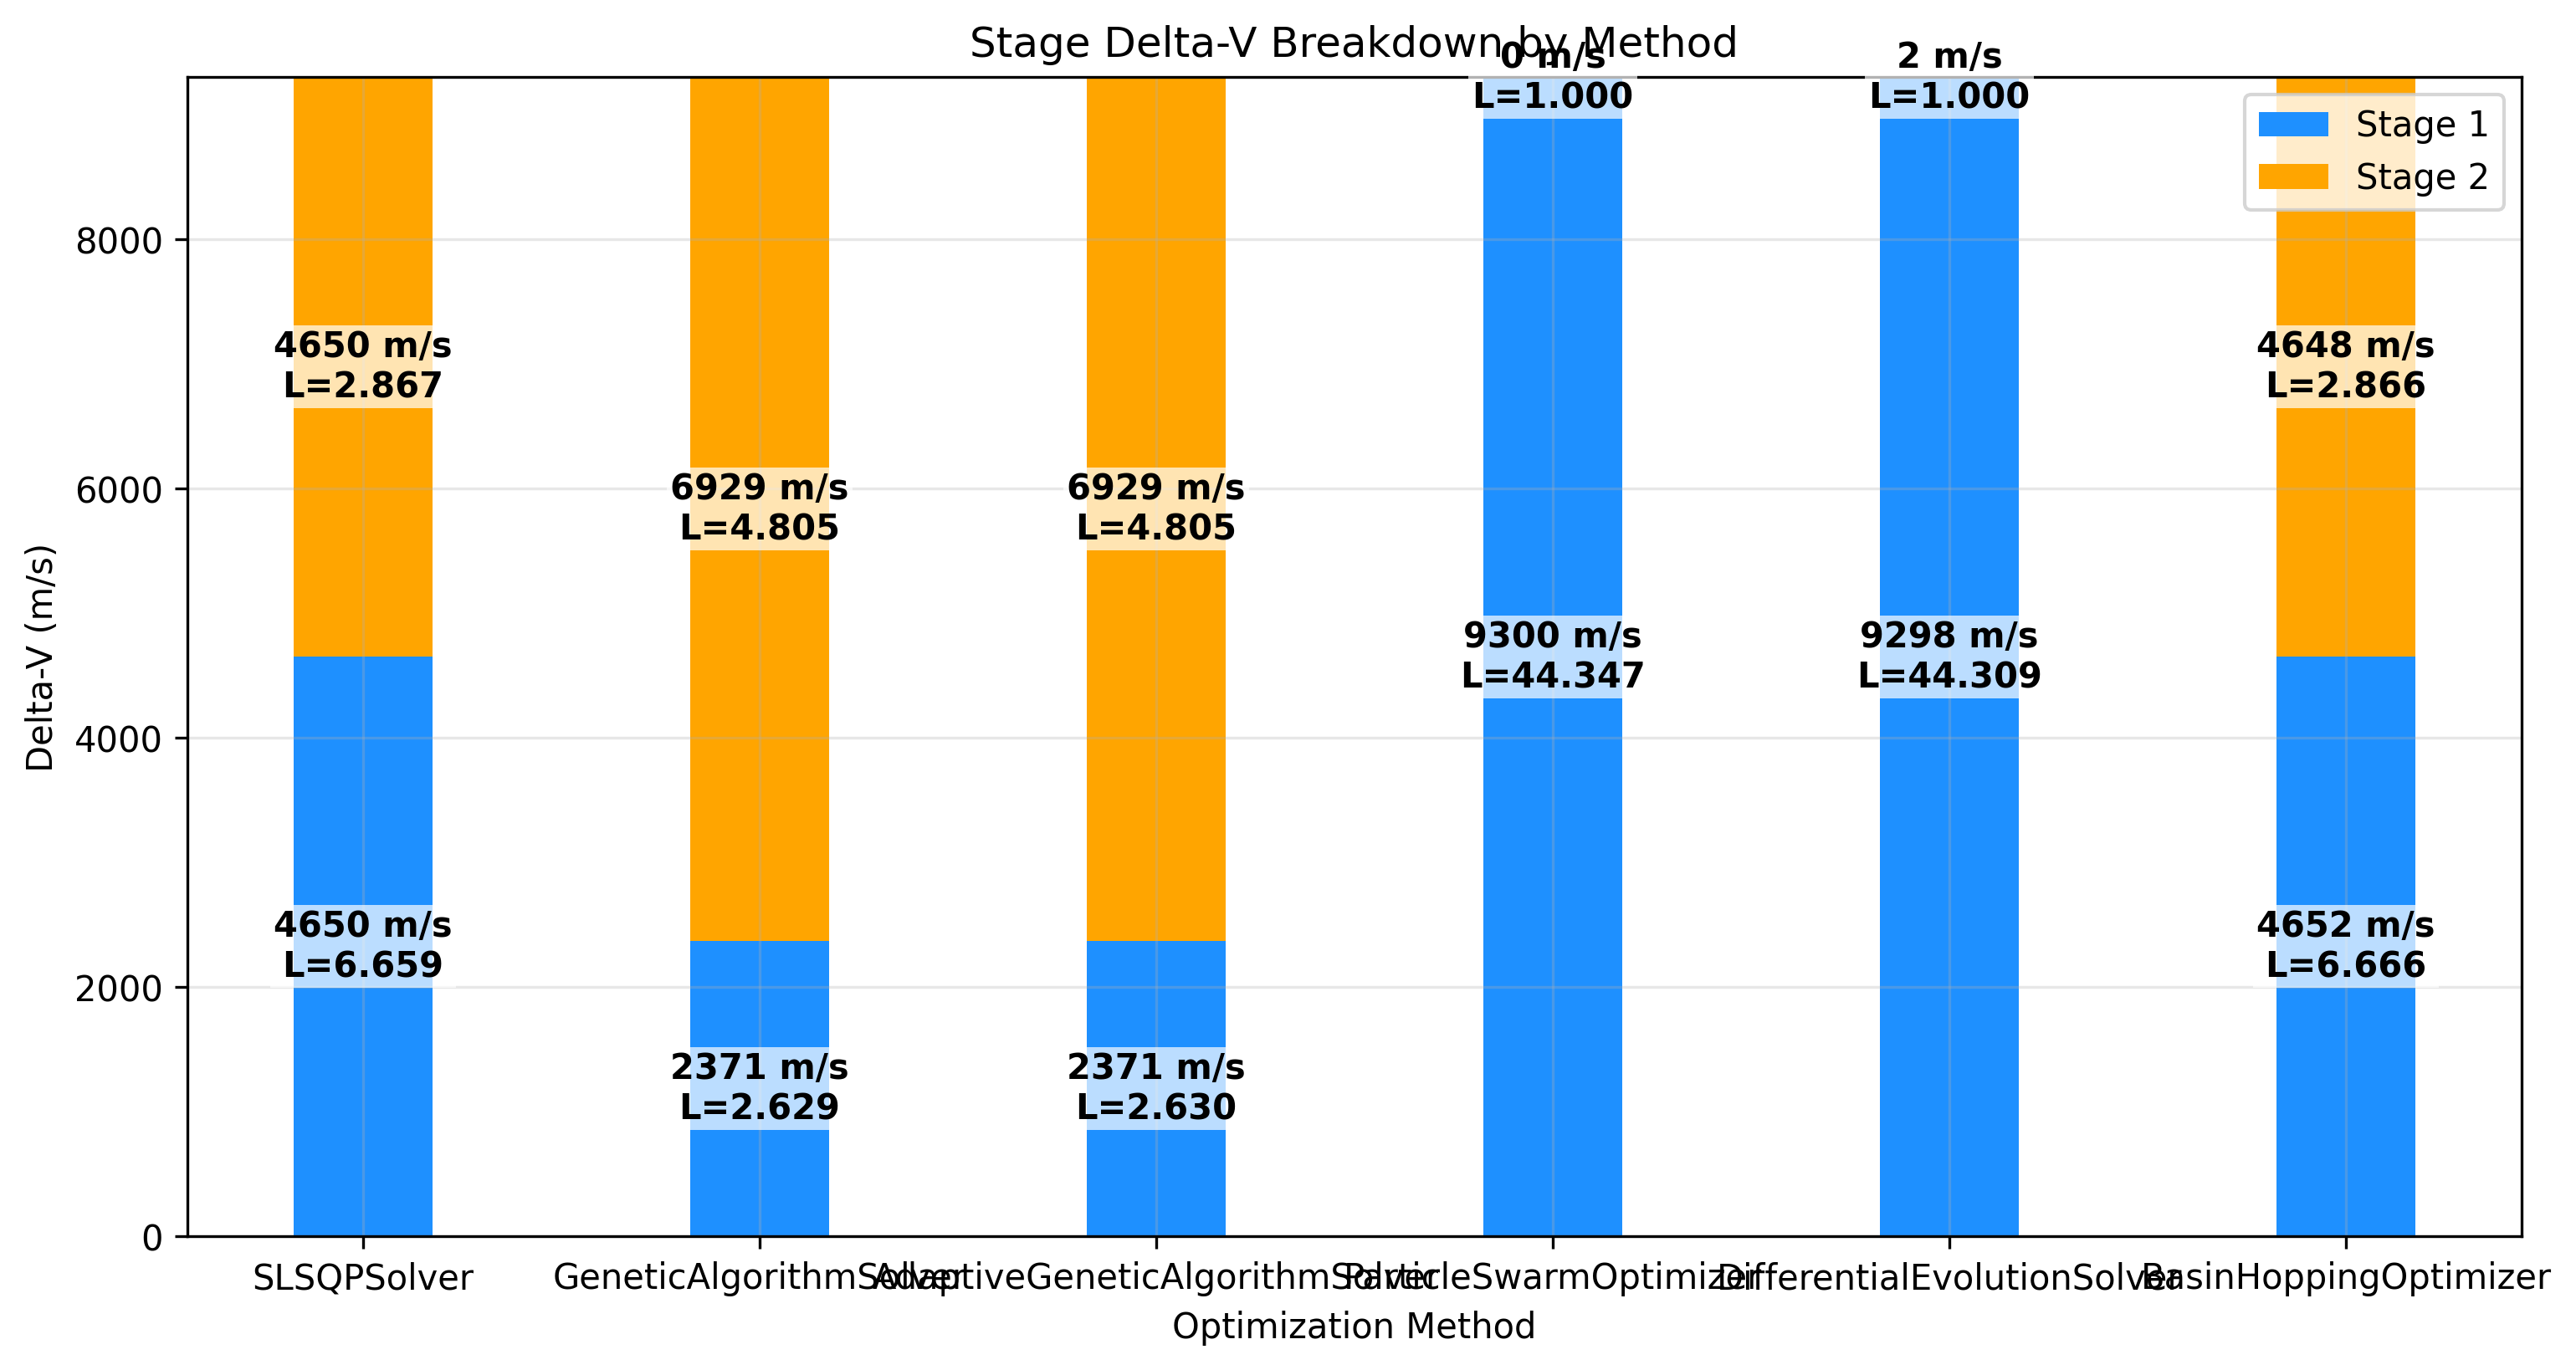
\includegraphics[width=\textwidth]{dv_breakdown.png}
\caption{$\Delta V$ Distribution Across Stages}
\end{figure}

\begin{figure}[H]
\centering
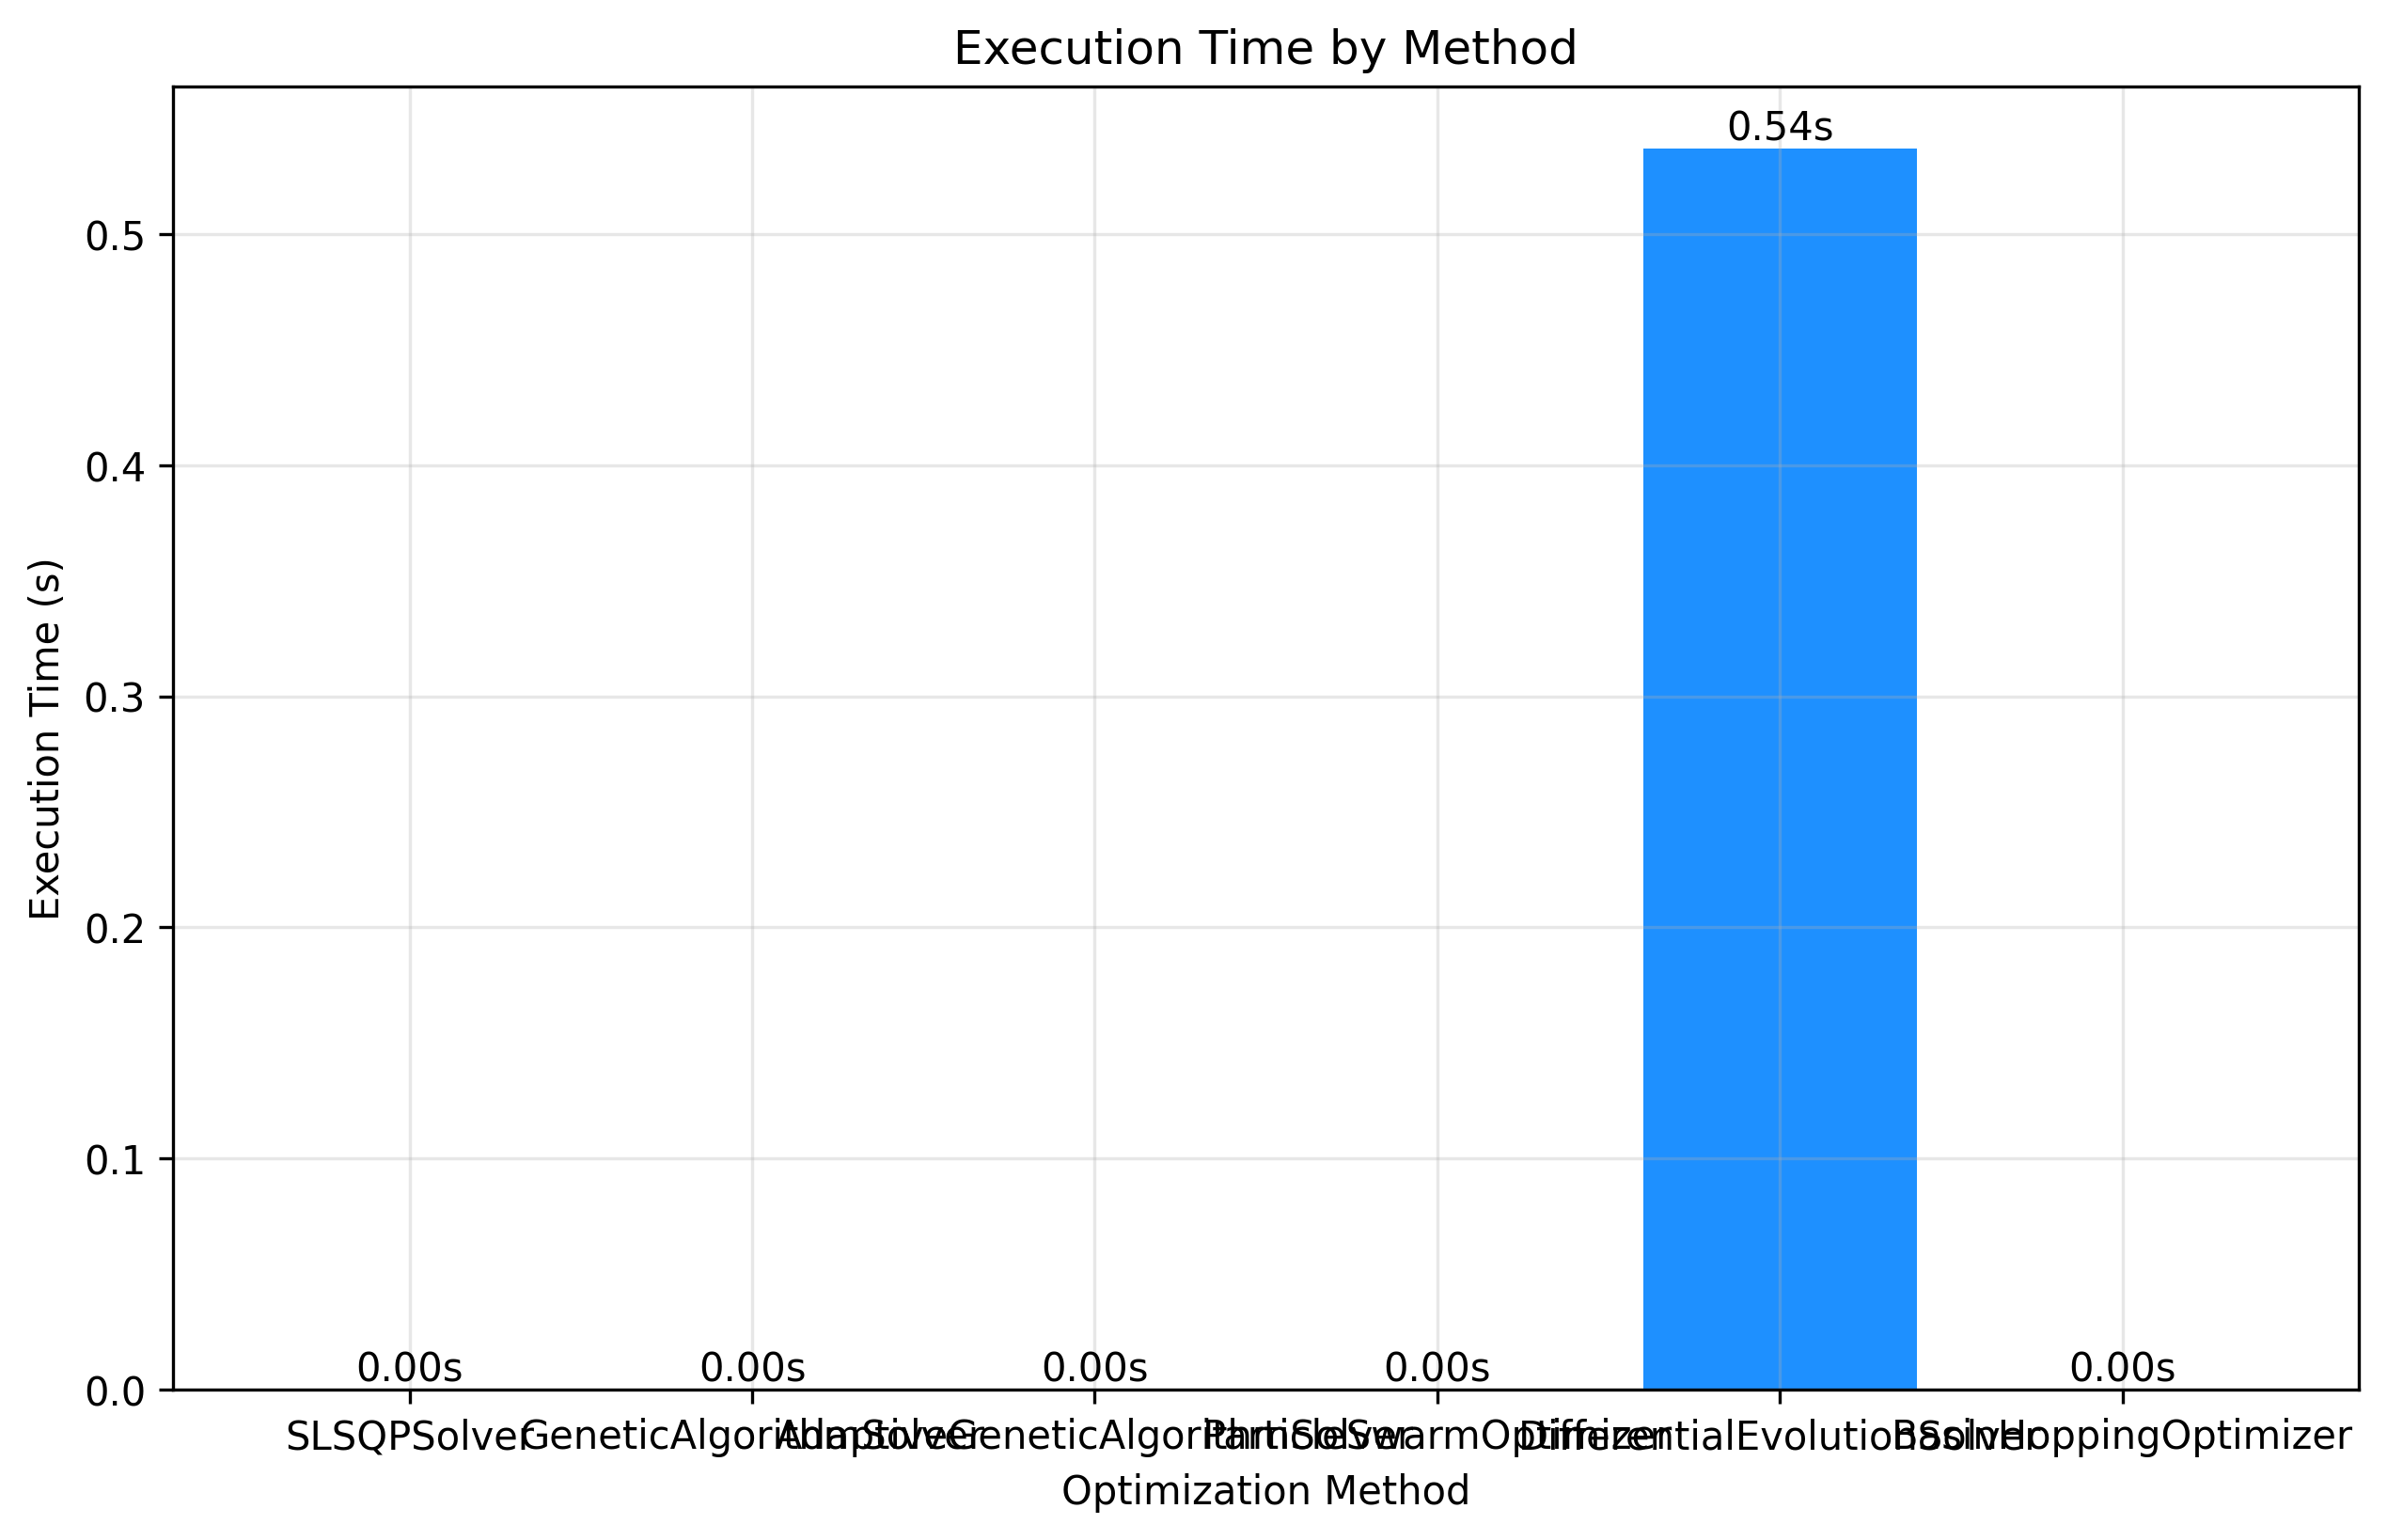
\includegraphics[width=\textwidth]{execution_time.png}
\caption{Solver Execution Time Comparison}
\end{figure}

\begin{figure}[H]
\centering
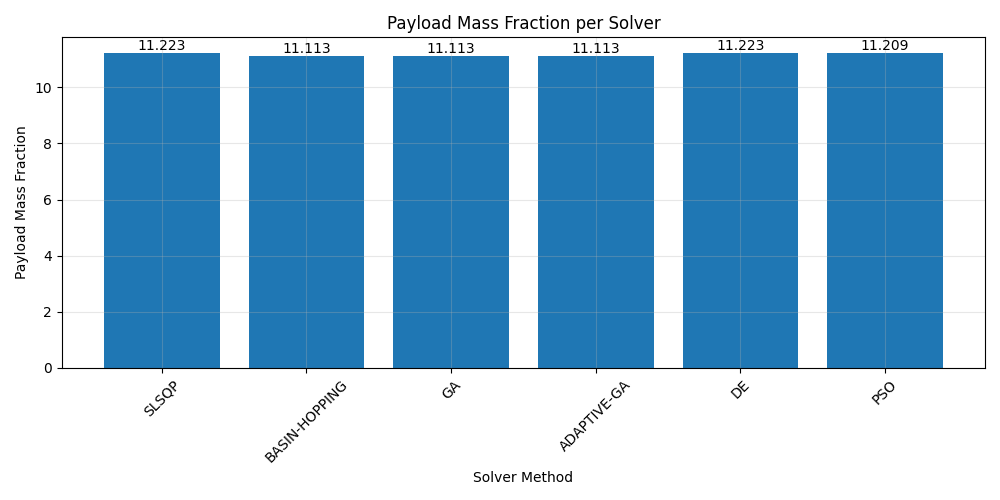
\includegraphics[width=\textwidth]{payload_fraction.png}
\caption{Payload Fraction Comparison}
\end{figure}

\section{Final Results Summary}
\begin{table}[H]
\centering
\caption{Optimization Results Summary}
\begin{tabular}{lccr}
\toprule
Method & Payload Fraction & Error & Time (s) \\
\midrule
SLSQP & 0.0073 & 0.0000e+00 & 0.00 \\
BASIN-HOPPING & 0.0073 & 0.0000e+00 & 1.41 \\
GA & 0.0151 & 0.0000e+00 & 3.25 \\
ADAPTIVE-GA & 0.0073 & 0.0000e+00 & 0.01 \\
DE & 0.0240 & 0.0000e+00 & 0.54 \\
PSO & 0.0240 & 0.0000e+00 & 0.45 \\
\bottomrule
\end{tabular}
\end{table}

\subsection{Detailed Stage Results}
\end{document}
